\documentclass[manuscript]{clv2}

%% \documentstyle[fullname]{article}

\usepackage{graphicx}  %%% for including graphics
\usepackage{url}       %%% for including URLs
%% \usepackage{fullname}

%% \documentclass[11pt]{article}
%% \usepackage{acl2012}
%% \usepackage{times}
%% \usepackage{latexsym}
%% \usepackage{multirow}
%% \usepackage{url}
%% \DeclareMathOperator*{\argmax}{arg\,max}
%% \setlength\titlebox{6.5cm}    % Expanding the titlebox

%\documentclass{svmult}

% % SVMult required packages
% \usepackage{mathptmx}
% \usepackage{helvet}
% \usepackage{courier}
% \usepackage{graphicx}
% \usepackage{makeidx}
% \usepackage{multicol}
% \usepackage{footmisc}


%\usepackage{url}
%\usepackage{latexsym}

\usepackage{amsmath}
\usepackage{amssymb}
%% \usepackage{amsthm}
\usepackage{color}
\usepackage{listings}
\usepackage{csvsimple}
\usepackage{graphicx}
\usepackage{fancyvrb}
%\usepackage{caption}
%\usepackage{subcaption}

%\renewcommand{\theTitleReference}[2]{\emph{#2}}

%% \renewcommand{\cite}{\citep}
%% \newcommand{\newcite}[1]{\citet{#1}}

%\newcommand{\citet}[1]{\citeauthor{#1} \shortcite{#1}}
%\newcommand{\citet}[1]{\cite{#1}}

%% \newtheorem*{theorem}{Theorem}
%% \theoremstyle{definition}
%% \newtheorem*{definition}{Definition}

\lstset{
  %basicstyle=\footnotesize\ttfamily, % Standardschrift
         basicstyle=\scriptsize\ttfamily, % Standardschrift
         %numbers=left,               % Ort der Zeilennummern
         numberstyle=\tiny,          % Stil der Zeilennummern
         %stepnumber=2,               % Abstand zwischen den
         %Zeilennummern
         numbersep=5pt,              % Abstand der Nummern zum Text
         tabsize=2,                  % Groesse von Tabs
         extendedchars=true,         %
         breaklines=true,            % Zeilen werden Umgebrochen
         keywordstyle=\color{black},
         frame=b,         
 %        keywordstyle=[1]\textbf,    % Stil der Keywords
 %        keywordstyle=[2]\textbf,    %
 %        keywordstyle=[3]\textbf,    %
 %        keywordstyle=[4]\textbf,   \sqrt{\sqrt{}} %
         stringstyle=\color{white}\ttfamily, % Farbe der String
         showspaces=false,           % Leerzeichen anzeigen ?
         showtabs=false,             % Tabs anzeigen ?
         xleftmargin=17pt,
         framexleftmargin=17pt,
         framexrightmargin=5pt,
         framexbottommargin=4pt,
         %backgroundcolor=\color{lightgray},
         showstringspaces=false,      % Leerzeichen in Strings anzeigen
         language=prolog
 }

\newcommand{\interp}[1]{[\![ #1 ]\!]}
\newcommand{\hide}[1]{}

\newcommand{\wfe}{\mbox{{\em wfe} }}
\newcommand{\wfes}{\mbox{{\em wfe}s }}

\newcommand{\newcite}[1]{\namecite{#1}}

\title{Efficiency in Ambiguity:\\ Two Models of Probabilistic Semantics for Natural Language}
\author{
       %% Daoud Clarke  \\
       %% University of Sussex, Brighton\\
       %% \texttt{daoud.clarke@gmail.com}
       %% \and
       %% Bill Keller  \\
       %% University of Sussex, Brighton\\
       %% \texttt{billk@sussex.ac.uk}
       }
\affil{}
\date{}

 \begin{document}
%\author{Daoud Clarke and Bill Keller}
% \institute{Daoud Clarke and Bill Keller \at Department of
% Informatics, University of Sussex, Falmer, Brighton,
% UK.\\ \email{\{d.clarke,~billk\}@sussex.ac.uk} }
\maketitle
\begin{abstract}
This paper explores theoretical issues in constructing an adequate probabilistic semantics for natural language. Two approaches are contrasted. The first extends Montague
Semantics with a probability distribution over 
models. It has nice theoretical properties, but does
not account for the ubiquitous nature of ambiguity; moreover inference is
NP-hard. An alternative approach is described in which a sequence of pairs of sentences and truth values is generated
randomly. By sacrificing some of the nice theoretical properties of
the first approach it is possible to model ambiguity naturally;
moreover inference now has polynomial time
complexity. Both approaches provide a compositional semantics and account for the gradience of semantic judgements of belief and inference.\footnote{The authors are grateful for the comments of a number of anonymous reviewers on earlier drafts. The work was funded as part of EPSRC EP/I037458/1, {\em A Unified Model of Compositional and Distributional Semantics: Theory and Applications\/.}}
%  are capable of modelling important features of
%  natural language semantics such as the reversal of entailment that
%  occurs with determiners such as ``all'' and ``no''.
\end{abstract}


% \begin{abstract}
%   Distributional accounts of meaning represent words as vectors or
%   probability distributions over contexts and differ markedly from
%   compositional, model-theoretic treatments of meaning such as
%   Montague semantics. Recently, researchers have begun to address the
%   problem of developing a unified account of natural language
%   semantics that combines the strengths of both the distributional and
%   compositional approaches. This paper proposes probabilistic
%   semantics as a basis of such a unifying account. 

%  % This paper argues for the adoption of
%  %  probabilistic semantics as a basis for such a unifying account. We
%  %  consider two different approaches. The first is a probabilistic
%  %  generalisation of Montague semantics in which we assume a
%  %  probability distribution over models. This approach has nice
%  %  theoretical properties but does not account for the ubiquitous
%  %  nature of ambiguity in natural language. This leads us to our second
%  %  approach, which we call \emph{Stochastic Semantics}, in which we
%  %  assume that a sequence of pairs of sentences and truth values are
%  %  generated randomly. We demonstrate that learning and inference are
%  %  feasible in both approaches, and that it is possible to learn that
%  %  certain quantifiers reverse the direction of entailment.
% \end{abstract}


\section{Introduction}

This paper explores theoretical  issues in developing an expressive and computationally tractable, probabilistic semantics for natural language.  Our general approach is situated within the formal, compositional semantics developed by Richard Montague, which is augmented to allow for probabilistic judgements about truth and inference. The present work takes  as a point of departure a number of key assumptions.
% %about the adequacy of a computational model of semantics for natural language. 
First, an adequate semantics should provide an account of both lexical and phrasal (i.e. compositional) meaning. Second, it should provide for judgements about degrees of belief. That is, a semantics should account for beliefs that statements are more or less likely to be true, or that one statement may entail another to a certain degree. Third, an adequate computational semantics should support effective procedures for learning semantic representations and for inference.

Vector space models of meaning have become a popular approach to computational semantics.
Distributional models represent word meanings as vectors of corpus-based distributional contexts and have been successfully applied to a wide variety of tasks, including, {\em inter alia\/}, word sense induction and disambiguation~\cite{khapra-EtAl:2010:ACL,Baskaya:13}, 
%prepositional phrase attachment~\cite{Calvo05distributionalthesaurus}, 
textual entailment~\cite{Marelli:14}, 
co-reference resolution~\cite{lee-EtAl:2012:EMNLP-CoNLL}
%, predicting semantic compositionality~\cite{bergsma-EtAl:2010:EMNLP} 
and taxonomy induction~\cite{fountain-lapata:2012:NAACL-HLT}. 
% % {\bf UPDATE THIS LIST??}
The success of vector-space models is due to several factors. They support fine-grained judgements of similarity, allowing us to account for semantic gradience, for example, that the lexeme {\em pear} is more similar to {\em banana}  than to, say, {\em cat}. Moreover, distributional vectors can be learnt in an unsupervised fashion from corpus data, either by counting occurrences of distributional contexts for a word or phrase, or by performing more sophisticated analysis on the data \cite{Mikolov:13,Pennington:14}. 

Vector-based approaches differ in many regards from compositional, model-theoretic treatments of meaning such as Montague semantics or Discourse Representation Theory \cite{Kamp:93}. It has proved challenging to extend vector space models to account for the way in which meanings may be composed and to support inference. The problem of developing a fully compositional, distributional semantics has recently become a very active area of research  \cite{Widdows:08,Mitchell:08,Baroni2010,Garrette:11,Grefenstette:11,Socher:12,Lewis:13} and efforts made to find a theoretical foundation \cite{Clarke:12,Kartsaklis:14}.  Researchers have also begun to address the problem of combining the strengths of both the distributional and model-theoretic approaches \cite{Clarke:07,Coecke:10,Garrette:11,Lewis:13}. 

This paper considers an alternative  strategy for developing a computational semantics. Starting with a compositional, model-theoretic semantics, this is augmented with ideas drawn from probabilistic semantics \cite{Gaifman:64,Nilsson:86,Sato:95}. Probabilistic semantics provides a rich seam of ideas that can be applied to the construction of a compositional semantics with desirable properties such as gradience and learnability. Below, we explore two different ways in which this might be achieved. Our objective is to map out some of the territory,  to consider issues of representational adequacy and computational complexity and to provide useful guidance for others venturing into this landscape. 

%In the first approach we define a probability distribution over Montague-style models in terms of a random generation process over interpretations. This provides the basis for a natural extension of Montague semantics to the probabilistic domain.  However, the approach embodies the assumption that whilst the meanings of words may vary between different interpretations, for any given interpretation they are fixed. This is clearly unrealistic: an adequate semantics should be capable of modelling cases where the interpretation of a given word varies across a text. Our second approach, which we call \emph{Stochastic Semantics}, addresses this restriction and allows for polysemy. Stochastic semantics assumes a random generative process for pairs of sentences and truth values, rather than models. As we show, this means that we have to sacrifice some nice theoretical properties satisfied by the first approach. However, the payoff is that in accounting for ambiguity,
%inference becomes more tractable since we can benefit from dynamic programming.

\hide{We show how to compute with both approaches, and show that both are
able to perform learning and inference on small examples. For example,
they can learn that while ``some cats $X$'' entails ``some animals
$X$'', entailment is reversed with other quantifiers: ``no animals
$X$'' entails ``no cats $X$''.}


%
%\subsection{Contributions}
%
%This paper explores theoretical properties of models of meaning. The
%reader may rightly question the value of a paper whose contributions
%are mainly theoretical in nature. Whilst we fully intend to explore
%our ideas in an experimental setting, we believe that readers who are
%interested in probabilistic approaches to natural language semantics
%will benefit from the theoretical ideas presented here. The reasons
%are as follows:
%\begin{itemize}
%\item We take a standard approach to natural language semantics
%  (Montague semantics) and augment it using a standard approach
%  (probabilistic semantics). We are thus in an area that seems natural
%  to explore.
%\item We are able to demonstrate deficiencies of this approach, both
%  in expressiveness and computational complexity, that may provide
%  useful guidance for others considering venturing into this
%  landscape.
%\item We identify an alternative area for exploration that alleviates
%  the difficulties associated with the first approach.
%\end{itemize}
%It is our hope that the ideas presented here can thus potentially save
%many wasted hours for those experimenting in this area. The specific
%contributions of this paper are as follows:
%\begin{enumerate}
%\item We show that Montague semantics can be combined with
%  probabilistic semantics by specifying a probability distribution
%  over Montague-style models.
%\item We show that it is possible to learn these probability
%  distributions directly from data by restricting the set of models,
%  whilst retaining many of the desirable properties of full Montague
%  semantics.
%\item We show that the problem of computing the probability that a
%  sentence is true is NP-hard.
%\item We show that taking account of lexical ambiguity leads to a new
%  model in which pairs of sentences and truth values are generated
%  randomly. The probability that a sentence is true can then be
%  computed in polynomial time.
%\item We show that both models are able to learn from a few examples
%  that quantifiers such as ``no'' reverse the direction of entailment.
%\end{enumerate}

% In the following we consider two different ways of constructing a
% probabilistic semantics. Both approaches have the following desirable
% properties:
% \begin{itemize}
% \item They are strongly grounded in probability theory: no ad-hoc methods
%   or heuristics are used to combine distributional semantics with
%   logical semantics.
% \item They admit an implementation in which probability distributions
%   can be learnt from data: the account is holistic, in that the
%   learning of word meaning and composition are not separated, with the
%   potential benefit of more flexible and accurate models of
%   compositional distributional semantics.
% \item Because both approaches describe a generative process,
%   composition does not necessarily lead to a loss of meaning (for
%   example by reducing the meaning of a sentence to a single truth
%   value).
% \end{itemize}

\section{Background}

\subsection{Montague Semantics}

In the early 1970s, 
%the linguist and philosopher 
Richard Montague detailed a formal treatment of natural language semantics \cite{Montague1970a,Montague1970b,Montague1973}. Montague's conception of semantics was truth-conditional and model-theoretic. He considered that a fundamental aim of any adequate theory of semantics was ``to characterise the notions of a true sentence (under a given interpretation) and of entailment'' \cite{Montague1970b}. A central methodological component of Montague's approach was the {\em Principle of Compositionality\/}: the meaning of an expression is a function of the meanings of its parts and the way they are combined syntactically.

Following Montague, we assume that natural language expressions
are parsed by a categorial grammar. Further,  every word has an
associated function with a type. Let $\mathcal{T}$ be the smallest set such that:
\begin{description}
\item [Basic types:] $e,t\in \mathcal{T}$
\item[Complex types:]  if $\alpha, \beta\in \mathcal{T}$, then $\alpha/\beta\in \mathcal{T}$.
\end{description}
Note that type $\alpha/\beta$ is the type of a function from type   $\beta$
to type $\alpha$.

The set $B$ of \emph{basic expressions} comprises
symbols denoting meanings of words. Each $b\in B$ has a type $\tau_b$. The set $\Lambda$ of
\emph{well-formed expressions}, and the extension of $\tau$ to $\Lambda$ are
defined as follows. Let $\Lambda$ be the smallest set such that:

\begin{itemize}
\item $B\subseteq \Lambda$
\item For every pair $\gamma,\delta\in \Lambda$ such that $\tau_\gamma
  = \alpha/\beta$ and $\tau_\delta = \beta$, then $\gamma(\delta)\in
  \Lambda$ and $\tau_{\gamma(\delta)} = \alpha$
\end{itemize}
Let $\Lambda_\tau$ denote the set of well-formed expressions of type
$\tau$. A \emph{sentence} is a well-formed expression of type $t$.

% An
% \emph{interpretation} is a function $\phi$ which assigns to every
% sentence a value of true or false, denoted $\top, \bot$ respectively.

The set $D_\tau$ of \emph{possible denotations} of type $\tau$ is
defined by:
\begin{eqnarray*}
D_e &=& E\\
D_t &=& \{\bot,\top\}\\
D_{\alpha/\beta} &=& {D_\alpha}^{D_\beta}
\end{eqnarray*}
where $E$ is a set of \emph{entities}. Thus the denotation of a
complex type is a function between the denotations for the types from
which it is composed. An \emph{interpretation} is a pair $\langle E,
F\rangle$ such that $E$ is a non-empty set and $F$ is a function with
domain $B$ such that $F(b) \in D_{\tau_b}$ for all $b\in B$. A well-formed expression $\gamma$ has the value $\interp{\gamma}$ in the
interpretation $\langle E, F\rangle$, where:
\begin{itemize}
\item $\interp{b} = F(b)$ for $b\in B$
\item $\interp{\gamma(\delta)} = \interp{\gamma}(\interp{\delta})$ for $\gamma
  \in \Lambda_{\alpha/\beta}$ and $\delta \in \Lambda_\beta$.
\end{itemize}
A sentence $s$ is \emph{true} in interpretation $\langle E, F\rangle$
if $\interp{s} = \top$, otherwise it is \emph{false}. A \emph{theory} $T$ is a set of pairs $(s,\hat{s})$, where $s$ is a
sentence and $\hat{s}\in\{\top,\bot\}$ is a truth value. A
\emph{model} for a theory $T$ is an interpretation $\langle E,
F\rangle$ such that $\interp{s} = \hat{s}$ for every sentence $s\in
T$. In this case we say that the model \emph{satisfies} $T$, and write
$\langle E, F\rangle \models T$.

\subsection{Probabilistic Semantics}
 
The idea of attaching probabilities to propositional truth is an old one and related to the foundation of probability itself
\cite{Keynes:21,Los:55}. \newcite{Gaifman:64} discusses probability measures for first order calculus; the work of \newcite{Sato:95}
concerns probability measures for logic programs. The idea we adopt is to associate probability measures with the space of models.
%% for the associated logic. 
Our approach is closely related in motivation to work by \newcite{Cooper:14}
%which proposes a semantics based on a probabilistic type theory.  The work reported here also shares common ground with recent work by
and \newcite{Goodman:14}.

%who argue strongly for the role of uncertainty in cognition and language understanding, whilst preserving a compositional, truth conditional semantics. They show how probability may be used to formalise uncertainty and the gradience of judgements about belief and inference and introduce a stochastic $\lambda$-calculus to provide compositional tools for probabilistic modeling of language and belief.


%To our knowledge, such measures have not been studied for
% higher order logics, which is what we consider here.

%A key idea in probabilistic semantics is to extend standard
%model-theoretic accounts of meaning by assuming a probability
%distribution over models.  

In model-theoretic semantics, a way to
view the meaning of a statement $s$ is as the set of all
interpretations $\mathcal{M}_s$ for which $s$ is true. 
%Interpretations
%in $\mathcal{M}_s$ are also called {\em models for\/} $s$. 
%Then $s$
%{\em logically entails\/} $t$ if and only if 
%%any model for $s$ is a
%%model for $t$: i.e. 
%$\mathcal{M}_s \subseteq
%\mathcal{M}_t$. 
Probabilistic semantics extends this idea by assuming
that models occur randomly.
%Informally, we may assume a probability
%distribution over the set of models. 
Formally, probabilities are defined in
terms of a probability space $\langle \Omega, \sigma, \mu\rangle$,
where $\Omega$ is the set of all models, $\sigma$ is a sigma algebra
associated with theories and $\mu$ is a probability measure on
$\sigma$.
We can then estimate the probability of a sentence $s$ as
the sum of the probabilities of all models $\mathcal{M}_s$, for $s$.

In general, the set of models will be infinite, but for purposes of 
exposition, consider a simple example with a small 
number of models, as in Table
\ref{table:models}. Each column defines a
different model of the relationship between John and Mary.  We
assume a probability distribution over models, with $P(m_1)
= 0.1$, $P(m_2) = 0.2$, $P(m_3) = 0.3$, $P(m_4) = 0.4$ (all other
possible models have probability zero). We can then
deduce the probability of statements about John and Mary:
\begin{itemize}
\item \emph{John likes Mary}: $\mu(\{m_2, m_3, m_4\}) = 0.9$
\item \emph{Mary likes John or Mary}: $\mu(\{m_1, m_3, m_4\}) = 0.8$
\item \emph{John likes Mary given that he loves her}: $$\mu(\{m_3, m_4\})/\mu(\{m_1, m_3, m_4\}) = 0.7/0.8$$
\end{itemize}


%\subsection{Example: Fine-grained Meanings}


% One distinguishing feature of distributional semantics is its ability
% to describe fine-grained aspects of meaning: the continuous nature of
% the space allows arbitrary degrees of similarity. We use the example
% from \cite{Clark:08}, computing the similarity of the two sentences
% \emph{John likes Mary} and \emph{John loves Mary}.

% We assume the following types for basic expressions:
% \begin{eqnarray*}
% \mathit{john},\mathit{mary} & \in & \Lambda_{(e/t)/t}\\
% \mathit{likes}, \mathit{loves} & \in & \Lambda_{(((e/t)/t)/((e/t)/t))/t}
% \end{eqnarray*}
% Proper nouns are interpreted as sets of sets of entities (functions
% from functions from entities to truth values to truth values), while
% verbs are functions from pairs of sets of sets of entities to truth
% values.

\begin{table}
  \begin{center}
  \begin{tabular}{l|l|l||c|c|c|c}
    \emph{subject} & \emph{verb} & \emph{object} & $m_1$ & $m_2$ & $m_3$ & $m_4$\\
    \hline
    john & likes & john & 1 & 1 & 1 & 1\\
    john & likes & mary & 0 & 1 & 1 & 1\\
    mary & likes & john & 1 & 0 & 0 & 1\\
    mary & likes & mary & 0 & 0 & 1 & 1\\
    john & loves & john & 1 & 1 & 1 & 1\\
    john & loves & mary & 1 & 0 & 1 & 1\\
    mary & loves & john & 1 & 1 & 1 & 1\\
    mary & loves & mary & 1 & 0 & 1 & 1\\
  \end{tabular}
  \end{center}
  \vspace{0.2cm}
  \caption{Four possible models describing relationships between John
    and Mary.}
  \label{table:models}
\end{table}

% \begin{table}
%   \begin{minipage}[b]{.5\linewidth}
%     % \centering
%     \label{table:models}
%   \end{minipage}%
%   \begin{minipage}[b]{.5\linewidth}
%     % \centering
%     \subcaption{Another subfigure}\label{fig:1b}
%   \end{minipage}
%   \caption{A figure}\label{fig:1}
% \end{table}

% For simplicity of exposition, and to make the number of
% interpretations we have to consider smaller, we will give some
% properties which will be fixed for all interpretations under
% consideration, i.e.~interpretations which do not satisfy the given
% property will be given probability zero. For example, we assume that
% the set $E$ of entities is fixed, $E = \{\mathbf{john},
% \mathbf{mary}\}$, and that the interpretation of nouns is fixed:
% $$\mathit{john}(x) = \begin{cases}
% \top & \text{if } x(\mathbf{john}) = \top\\
% \bot & \text{otherwise}
% \end{cases}$$ i.e.~$\mathit{john}$ is the set of all sets containing
% the entity $\mathbf{john}$, and similarly for $\mathit{mary}$, if we
% interpret functions with range $\{\top,\bot\}$ as indicator
% functions. We further assume that $\mathit{likes}$ and
% $\mathit{loves}$ behave logically so that if ``John likes $x$'' is
% true and ``Mary likes $x$'' is true then ``John and Mary like $x$'' is
% also true (note that this isn't true for all verbs; consider ``John
% and Mary played chess''). Similarly we assume that if ``$x$ likes
% John'' and ``$x$ likes Mary'' are true then ``$x$ likes John and
% Mary'' is true.

% Four possible models $m_1, m_2, m_3, m_4$ under these assumptions are
% described in Table \ref{table:models}. At this point our example
% diverges from standard model-theoretic semantics. 


% We assume that the categorial grammar assigns the meaningful
% expression $\mathit{likes}(\mathit{mary})(\mathit{john})$ to the
% sentence ``John likes Mary''. The probability of this sentence is
% \begin{eqnarray*}
% \mu(M(\{\mathit{likes}(\mathit{mary})(\mathit{john})\})) &=&
% \mu(\{m_2, m_3, m_4\})\\
% &=&0.9
% \end{eqnarray*}
% Similarly, the models which are true for the sentence ``John loves
% Mary'' are $\{m_1, m_3, m_4\}$, having probability 0.8. The models
% which satisfy both of these sentences are $\{m_3, m_4\}$ with
% probability 0.7, so the
% degree to which ``John loves Mary'' entails ``John likes Mary'' is
% $0.7/0.8$. Note that in this case there is no logical entailment, but
% there is a high degree of entailment.

% \subsection{Example: Conjunction and Disjunction}

% Our formalism inherits the nice properties of model-theoretic
% semantics with respect to conjunction and disjunction. We describe the
% conjunction of nouns with the basic expression $\mathit{and}$ of type
% $(((e/t)/t)/((e/t)/t))/((e/t)/t)$: it is a function taking two sets of
% sets of entities, and returning another set of sets of
% entities. Specifically we assume that it returns the intersection of
% the two sets. Similarly $\mathit{or}$ is a function of the same type,
% returning the union of the two sets.

% Then $\mathit{and}(john)(mary)$ is the set of sets containing both
% $\mathbf{john}$ and $\mathbf{mary}$. Assume the categorial grammar
% gives the meaningful expression
% $\mathit{likes}(\mathit{and}(\mathit{john})(\mathit{mary}))(\mathit{mary})$
% to the sentence ``Mary likes John and Mary''. The set of models
% satisfying this sentence is $\{m_4\}$, so this sentence has
% probability 0.4. The set of models satisfying
% $\mathit{likes}(\mathit{or}(\mathit{john})(\mathit{mary}))(\mathit{mary})$
% for ``Mary likes John or Mary'' is $\{m_1, m_3, m_4\}$, so this
% sentence has probability 0.8. Note that the logical entailments we
% would expect from logical semantics are preserved: the degree to which
% ``Mary likes John and Mary'' entails ``Mary likes John'' is 1.

%  In this example, we
% assume that meanings are described by a measure space for each part of
% speech. Measure spaces for larger constituents are then constructed as
% product measures \cite{Taylor:06} of their constituent measure
% spaces. This idea is an extension of the observation of
% \citet{Keenan:85} that there is a Boolean algebra associated with each
% constituent.

% A measure space can be constructed for a particular part of speech
% directly from the distributional semantic representations of the
% associated words, or from an ontology with frequency information
% \cite{Clarke:07}.


\section{A Probabilistic Montague Semantics}

Let $\Omega$ be the set of all Montague-style interpretations,  $M(T)$ the set of all models for the theory $T$ and
$\sigma_0$ the set of all sets of models that satisfy some theory: $\sigma_0 = \{M(T) : T\text{ is a theory}\}$.
In general, $\sigma_0$ is not a sigma algebra, as it is not
guaranteed for any two theories $T_1$, $T_2$ that
$M(T_1)\cup M(T_2) \in \sigma_0$. For any Montague grammar containing a propositional
fragment  this would hold, but even if this is not the case we
can still define a probability space by considering the sigma algebra
$\sigma$ generated by $\sigma_0$: the smallest
sigma algebra containing $\sigma_0$. For $\mu$ a probability measure on $\sigma$, 
$\langle\Omega,\sigma,\mu\rangle$ is a probability space
describing the probability of theories. The probability of $T$ is defined as
$\mu(M(T))$. For  sentences $s_1$ and $s_2$ such that $\mu(M(\{(s_2,\top)\}) >0$, the conditional
probability $P(s_1 | s_2 )$  is interpreted as the {\em degree to which $s_2$ entails $s_1$\/} and defined as
$$ P(s_1|s_2) = \frac{\mu(M(\{(s_1, \top), (s_2, \top)\}))}{\mu(M(\{(s_2,\top)\}))}$$
Note too that for $\mu(M(\{(s_2,\top)\})) > 0$, if $s_2$ {\em logically entails\/} $s_1$, then
$P(s_1|s_2) = 1$.


%%the degree to which  $s_2$ entails $s_1$ is $1$.

% A \emph{theory} is a set $T$ of pairs $(s,\hat{s})$, where $s$ is a
% sentence and $\hat{s}\in\{\top,\bot\}$ is a truth value. A
% \emph{model} for a theory $T$ is an interpretation which assigns
% $\hat{s}$ to every sentence $s\in T$. In this case we say that the model \emph{satisfies} $T$. Let $\Omega$ be the set of all
% interpretations, and $\sigma$ be the sigma algebra consisting of the
% set of all sets of models that satisfy some theory. Let $\mu$ be a probability measure
% on $\sigma$; then $\langle\Omega,\sigma,\mu\rangle$ is a probability
% space which describes the probability of theories. Let $M(T)$ denote
% the set of all models for the theory $T$; the probability of $T$ is
% $\mu(M(T))$.


% In this paper, we consider the situation where the logical language
% $L$ is restricted to that of logic programs, i.e.~Horn clauses with
% universal quantification, and we use Herbrand models. In this case,
% the distribution can be defined in terms of minimal models, as
% demonstrated by Sato (\citeyear{Sato:95}), meaning that probabilities
% of logical sentences can be computed efficiently. He also shows that
% in this case distributions can be efficiently learnt from data using
% the Expectation Maximisation (EM) algorithm. We demonstrate how this
% can work for toy data consisting of natural language sentences.

%\section{Learning}

%\section{Examples}

% One can envisage many possible ways of describing probability measures
% $\mu$. Our main goal is to be able to learn such measures from corpus
% data, and we describe one possible approach to doing this in Section
% \ref{section:distributions}. However, in this section, to demonstrate
% the potential for our approach, we give examples in which measures are
% given explicitly.
 
\subsection{Restricting the Space of Models}
\label{section:distributions}

A key objective is to be able to learn semantics from corpus data.  We describe one way this may be achieved within our
framework. The central idea is to limit the number of denotations
under consideration and define a probabilistic generative model for
interpretations. Assume $E$ is fixed. Let
$\phi_\tau = \{\interp{\lambda} : \lambda\in \Lambda_\tau\}$ be the
set of denotations occurring with type $\tau$. Assume $F$ is
constrained s.t. $|\phi_\tau| = n_\tau$, where $n_\tau$ is a
constant for each type satisfying $n_\tau \le |D_\tau|$. Note that
$\phi_\tau \subseteq D_\tau$ and $\phi_\tau$ can be a lot smaller
than $D_\tau$ if the range of $F$ restricted to $\Lambda_\tau$ does
not cover all of $D_\tau$.  We also assume that the occurring
denotations are ordered, so we can write $\phi_\tau =
\{d_{\tau,1}, d_{\tau,2}, \ldots d_{\tau, n_\tau}\}$.
The restriction in the number of occurring denotations makes learning
a distribution over models practicable, since the space of exploration
can be made small enough to handle in a reasonable amount of time.

We assume that denotations are generated with probabilities
conditionally independent given a random variable taking values from
some set $H$. This gives us the following process to generate $F$:
\begin{itemize}
\item Generate a hidden value $h\in H$ where $P(h) = \theta_h$
\item Generate $F(b) \in \phi_{\tau_b}$ for each $b\in B$ where
  $P(d_{\tau_b,i}|b, h) = \theta_{b,i,h}$
\item Generate $d_{\alpha/\beta,i}(d_{\beta,j}) \in \phi_\beta$ for each $d_{\alpha/\beta,i}$, $d_{\alpha,j}$,
where $P(d_{\beta,k}|d_{\alpha/\beta,i}, d_{\alpha,j},h) = \theta_{\alpha,\beta,i,j,k,h}$
%\begin{itemize}
%\item Generate a value $\interp{d_{\alpha/\beta,i}(d_{\alpha,j})}$
%  according to $P(d_{\beta,k}|d_{\alpha/\beta,i}, d_{\alpha,j},h) = \theta_{\beta,i,j,k,h}$
%\end{itemize}
\end{itemize}
The parameters to be learnt are the probability distributions
$\theta_h$ over hidden values, $\theta_{b,i,h}$ over possible values
$d_{\tau_b,i}$, for each basic expression $b$ and hidden value $h$,
and $\theta_{\alpha,\beta,i,j,k,h}$ over values $d_{\beta,k}$ for each
function $d_{\alpha/\beta,i}$, argument $d_{\beta,j}$ and hidden
value $h$.

\subsection{Example}

As an example, we show a restricted probabilistic Montague semantics
which mimics the semantics of standard propositional logic. Although
our intended application is natural language semantics, and
probabilities are supposed to be inferred from data rather than
specified in a table as we do here, this example will be used later to
demonstrate that inference for this formalism is NP-hard. Hidden
values are not needed, so assume $H$ has a single element.

We use the following basic expressions: variables $P_i$ of type $t$,
and logical symbols $\land$ and $\lor$ of type $(t/t)/t$ and $\lnot$
of type $t/t$. For example $\land (P_1)(\lnot (P_2))$ is a sentence
which, using a more familiar notation, might be written as $P_1 \land
\lnot P_2$.

The possible denotations for each type and their associated
probabilities are shown in Table \ref{table:pmsat}. In this example,
each variable $P_i$ can take the value $\top$ or $\bot$ with equal
probability. This means that any sentence has a non-zero probability
if and only if it is satisfiable. Every other denotation in this
example is deterministic (since all other values in the table are 0 or
1); these simply serve to reproduce the familiar truth tables of
logic. We use symbols instead of numeric subscripts for the
denotations to give a better intuition as to their purpose. For
example, $d_{t/t,I}$ acts as the identity on truth values, and
$d_{t/t,\lnot}$ acts as negation.

\begin{table}
\hfill
\begin{tabular}{c|c|c}
 & $\top$ & $\bot$ \\
\hline
$\interp{P_i}$ & 0.5 & 0.5 \\
$d_{t/t,I}(\top)$ & 1 & 0\\
$d_{t/t,I}(\bot)$ & 0 & 1\\
$d_{t/t,\top}(\top)$ & 1 & 0\\
$d_{t/t,\top}(\bot)$ & 1 & 0\\
$d_{t/t,\bot}(\top)$ & 0 & 1\\
$d_{t/t,\bot}(\bot)$ & 0 & 1\\
$d_{t/t,\lnot}(\top)$ & 0 & 1\\
$d_{t/t,\lnot}(\bot)$ & 1 & 0
\end{tabular}\hfill
\begin{minipage}[c][4.3cm]{0.5\linewidth}
\centering
\begin{tabular}{c|c|c|c|c}
 & $d_{t/t,I}$ & $d_{t/t,\top}$ & $d_{t/t,\bot}$ & $d_{t/t,\lnot}$ \\
\hline
$\interp{\lnot}$ & 0 & 0 & 0 & 1 \\
$d_{(t/t)/t,\lor}(\top)$ & 0 & 1 & 0 & 0\\
$d_{(t/t)/t,\lor}(\bot)$ & 1 & 0 & 0 & 0\\
$d_{(t/t)/t,\land}(\top)$ & 1 & 0 & 0 & 0\\
$d_{(t/t)/t,\land}(\bot)$ & 0 & 0 & 1 & 0\\
\end{tabular}%
\vfill
\begin{tabular}{c|c|c}
 & $d_{(t/t)/t,\land}$ & $d_{(t/t)/t,\lor}$ \\
\hline
$\interp{\land}$ & 1 & 0 \\
$\interp{\lor}$ & 0 & 1 \\
\end{tabular}%
\end{minipage}%
\hspace*{\fill}
\vspace{0.2cm}
\caption{Probabilities of a restricted probabilistic Montague
  semantics to demonstrate NP-hardness of PM-SAT. Each column shows
  the probability of generating a particular denotation.}
\label{table:pmsat}
\end{table}



\subsection{Learning and Inference}

For a theory $T$ and parameters $\theta$, we compute $P(T|\theta)$ as follows. For each hidden variable $h$:
%\begin{itemize}
%\item For each hidden variable $h$:
\begin{itemize}
\item Iterate over models for $T$. This can be done bottom-up
  by first choosing the denotation for each basic expression,
  then recursively for complex expressions. Choices must be
  remembered and if a contradiction arises, the
  model is abandoned.
\item The probability of each model given $h$ can be found by
  multiplying the parameters associated with each choice made in the
  previous step.
\end{itemize}
%\end{itemize}

We can use Maximum Likelihood to estimate the parameters given a set
of observed theories $\mathcal{D} = \{T_1, T_2, \ldots T_N\}$. We look
for the parameters $\theta$ that maximize the likelihood
$$P(\mathcal{D}|\theta) = \prod_{n=1}^N P(T_i|\theta)$$ This can be
maximised using gradient ascent or expectation maximisation. We have
verified that this can be done for small examples with a simple Python
implementation.

\section{Stochastic Semantics}

Our formulation of Probabilistic Montague Semantics
does not adequately account for ambiguity in natural language.
Although we have a probability distribution over
interpretations, 
in any given interpretation each occurrence of a
word must have the same denotation. This is unsatisfactory, as a
word may exhibit different senses across a
theory. For example, consider two sentences, each
containing  an occurrence of the word \emph{bank}, but with different senses. In our current
formulation both occurrences of \emph{bank} are forced to have the same denotation. To allow
a word's meaning 
to vary across a theory, one possibility
is to represent
different occurrences of a word by different
predicates. For example, we might perform word sense disambiguation on
each sentence and decide that the two occurrences of \emph{bank} are
unrelated. In this case, the first occurrence might be
represented by the predicate {\em bank}$_1$ and the second by {\em
  bank}$_2$.


%%  This approach
%% assumes the existence of some additional learning mechanism for
%% acquiring word senses, quite separate from that employed to learn
%% model parameters.


We consider an alternative which incorporates \emph{degrees of ambiguity} into the representation of a word's meaning. This is consistent with many distributional  frameworks, where a word is often represented as a vector of all of its contexts of occurrence, regardless of sense. 
We drop the requirement that in any given interpretation, each occurrence of a word must have the same denotation. Generalising this idea to denotations for all types results in an entirely different semantic model. It turns out that this model can be formulated in a straightforward way within the framework due to \newcite{Sato:97}. We call our new framework \emph{Stochastic Semantics}.  We no longer
associate a set of models with a sentence, but instead assume that pairs of sentences and
truth values are randomly generated in sequence. The probability of
each pair being generated is conditionally independent of previous
pairs given the hidden variable.

% in which we have a probability distribution over
% \emph{theories} instead of models. We can define a generative
% model for theories, analogous to the one for models, as follows:
% \begin{itemize}
% \item Choose a hidden value $h$
% \item Choose a number $n$ of sentences according to some distribution
%   (e.g. Poisson)
% \item Do $n$ times:
% \begin{itemize}
% \item For each basic expression occurrence $b$ in $s$, generate a
%   value in $\phi_{\tau_b}$ according to $P(d_{\tau_b,i}|b, h) =
%   \theta_{b,i,h}$
% \item For each expression of the form $\gamma(\delta)$, where $\gamma$
%   and $\delta$ have values $d_{\tau_\gamma,i}$ and $d_{\tau_\delta,j}$
%   respectively, choose a value in $\phi_{\tau_{\gamma(\delta)}}$
%     according to $P(d_{\tau_{\gamma(\delta)},k}|d_{\tau_\gamma,i},
%       d_{\tau_{\delta},j}) = \theta_{\tau_{\gamma(\delta)},i,j,k,h}$
% \end{itemize}
% \end{itemize}

\begin{figure}
\centering
\begin{lstlisting}
% Hidden variable
values(hidden, [h0, h1]).

% Types
values(word(noun, Word, Hidden), [n0, n1]).
values(word(verb, Word, Hidden), [v0, v1]).
values(word(det, Word, Hidden), [d0, d1]).
values(function(s, Value1, Value2, Hidden), [t0, t1]).
values(function(np, Value1, Value2, Hidden), [np0, np1]).
values(function(vp, Value1, Value2, Hidden), [vp0, vp1]).

evaluate(w(Word, Type), Hidden, Result) :-
	msw(word(Type, Word, Hidden), Result).
evaluate(f(Type, X, Y), Hidden, Result) :-
	evaluate(X, Hidden, XResult),
	evaluate(Y, Hidden, YResult),
	msw(function(Type, XResult, YResult, Hidden), Result).

theory([], _).
theory([truth(Sentence, Result)|Tail], Hidden) :-
	evaluate(Sentence, Hidden, Result),
	theory(Tail, Hidden).

theory(T) :-
	msw(hidden, Hidden),
	theory(T, Hidden).
\end{lstlisting}
\caption{A PRISM program describing probability distributions over
  natural language models used for our examples.}
\label{figure:program}
\end{figure}

%% \begin{figure}
%% \begin{lstlisting}
%% :- prob(theory([
%%   truth(f(s, f(np, w(the, det),
%%                    w(cat, noun)),
%%              f(vp, w(likes, verb),
%%                    f(np, w(the, det),
%%                          w(dog, noun)))),
%%         t1)]), X).
%% \end{lstlisting}
%% \caption{PRISM query to evaluate the probability that the sentence
%%   \emph{the cat likes the dog} is true.}
%% \label{figure:query}
%% \end{figure}



%\subsection{Implementation}

An illustrative implementation of Stochastic Semantics is shown in Figure \ref{figure:program}. The code is written in PRISM  \cite{Sato:97}, a probabilistic extension of the Prolog logic-progamming language that incorporates probabilistic predicates and declarations. In particular, PRISM allows {\em random switches}. In the code, the predicate \texttt{values} is used to declare a named switch and associate with it a number of possible outcomes. The probabilistic predicate \texttt{msw} allows a random choice to made amongst these outcomes at execution time. To simplify the code, complex types of the grammar are referred to by their corresponding natural language
categories: type $t$ is represented by \texttt{s}, type $(t/e)$ by \texttt{vp} and type $t/(e/t)$ by \texttt{np}. 

The program defines how sentences are randomly assigned truth values. For example, the switch
%% \vspace*{-0.8cm}
%\begin{center}
\texttt{values(word(noun,Word,Hidden),[n0,n1])} 
%\end{center}
introduces a switch for nouns having two possible outcomes, \texttt{n0} and \texttt{n1}.
The outcomes are conditioned on the particular choice of noun (\texttt{Word}) and on the choice of hidden variable (\texttt{Hidden}). Similarly, switches are associated with complex types. For example the values associated with a sentence (\texttt{s}) switch are conditioned on the choices of its component parts and a hidden variable, and so on.

The probability of a theory is derived by evaluating the truth
conditions of its component sentences.
%that make it up.\hide{
Note that probability
distributions are defined over models, not theories, so that to
evaluate the probability of a theory it is necessary to sum over the
probabilities of all of its satisfying models. To achieve this, the
predicate \texttt{prob} is used.
For example, a query returning the
probability of the sentence {\em the cat likes the dog\/} would be expressed as a theory
$\{(\mathit{likes}(\mathit{the}(\mathit{dog}))(\mathit{the}(\mathit{cat})),\top)\}$,
which can be translated into a Prolog expression in a straightforward
manner:
\begin{Verbatim}[fontsize=\small]
:- prob(theory([truth(f(s,
    f(np, w(the, det), w(cat, noun)),
    f(vp, w(likes, verb), f(np, w(the, det), w(dog, noun)))),
  t1)]), X).
\end{Verbatim}



\section{Complexity}

We focus on determining the probability of a sentence,
as this is needed for both learning and inference.

\subsection{Complexity of Probabilistic Montague Semantics}

We first consider the problem of {\em Probabilistic Montague Semantics satisfiability\/} (PM-SAT) and then show that the problem of computing the probability of a sentence must be at least as hard.

\begin{definition}[PM-SAT]

  Given 
%  a restricted probabilistic
%  Montague semantics for a language, that is, 
  a restricted set of
  denotations $\phi_\tau$ for each type $\tau$ and probability
  distributions defined by $\theta$, determine whether the probability
  of a given sentence taking the value $\top$ is non-zero.
\end{definition}

\begin{theorem}
  \emph{PM-SAT} is NP-complete with respect to the length of the input
  sentence.
\end{theorem}

%\begin{table}
%\hfill
%\begin{tabular}{c|c|c}
% & $\top$ & $\bot$ \\
%\hline
%$\interp{x_i}$ & 0.5 & 0.5 \\
%$d_{t/t,I}(\top)$ & 1 & 0\\
%$d_{t/t,I}(\bot)$ & 0 & 1\\
%$d_{t/t,\top}(\top)$ & 1 & 0\\
%$d_{t/t,\top}(\bot)$ & 1 & 0\\
%$d_{t/t,\bot}(\top)$ & 0 & 1\\
%$d_{t/t,\bot}(\bot)$ & 0 & 1\\
%$d_{t/t,\lnot}(\top)$ & 0 & 1\\
%$d_{t/t,\lnot}(\bot)$ & 1 & 0
%\end{tabular}\hfill
%\begin{minipage}[c][4.6cm]{0.5\linewidth}
%\centering
%\begin{tabular}{c|c|c|c|c}
% & $d_{t/t,I}$ & $d_{t/t,\top}$ & $d_{t/t,\bot}$ & $d_{t/t,\lnot}$ \\
%\hline
%$\interp{\lnot}$ & 0 & 0 & 0 & 1 \\
%$d_{t/(t/t),\lor}(\top)$ & 0 & 1 & 0 & 0\\
%$d_{t/(t/t),\lor}(\bot)$ & 1 & 0 & 0 & 0\\
%$d_{t/(t/t),\land}(\top)$ & 1 & 0 & 0 & 0\\
%$d_{t/(t/t),\land}(\bot)$ & 0 & 0 & 1 & 0\\
%\end{tabular}%
%\vfill
%\begin{tabular}{c|c|c}
% & $d_{t/(t/t),\land}$ & $d_{t/(t/t),\lor}$ \\
%\hline
%$\interp{\land}$ & 1 & 0 \\
%$\interp{\lor}$ & 0 & 1 \\
%\end{tabular}%
%\end{minipage}%
%\hspace*{\fill}
%\caption{Probabilities of a restricted probabilistic Montague
%  semantics to demonstrate NP-hardness of PM-SAT. Each column shows
%  the probability of generating a particular denotation.}
%\label{table:pmsat}
%\end{table}

\begin{proof}
The example of restricted Montague semantics described above has the
property that a sentence has a non-zero probability if and only if it
is satisfiable. Note for example that there is an interpretation for
which $\land (P_1)(\lnot (P_2))$ has value $\top$. From Table
\ref{table:pmsat} we can see that this sentence has probability 0.25,
from the case where $P_1$ takes the value $\top$ and $P_2$ takes the
value $\bot$. On the other hand, the sentence $\land (P_1)(\lnot
(P_1))$ will have value $\bot$ for all interpretations and thus has
probability 0. Hence we can solve SAT if we can solve PM-SAT, and so
PM-SAT is NP-hard.

Finally, to show NP-completeness we note that PM-SAT can be solved by
a non-deterministic machine in time linear in sentence length. This is
achieved by choosing a value from $H$, assigning every possible value
to all basic expressions and then recursively to complex
expressions. Any assignment that gives a non-zero probability for the
sentence taking the value $\top$ will return true. So PM-SAT is in NP
and is thus NP-complete.
\end{proof}

Let us call the problem of computing the probability of a sentence in
Probabilistic Montague Semantics PM-PROB. Clearly PM-PROB is at least
as hard as PM-SAT, since if we knew the probability of a sentence we
would know whether it was non-zero. It follows that PM-PROB is NP-hard.

\subsection{Complexity of Stochastic Semantics}

Let us call the problem of computing the probability of a sentence for Stochastic Semantics, SS-PROB. We show that SS-PROB is computationally easier than PM-PROB.
Note that for Stochastic Semantics there is no dependency between different parts of a sentence.
%Given a fixed hidden value, the probability
%of a sentence can thus be computed more efficiently than for
%Probabilistic Montague Semantics. 
Dynamic
programming can then be used to store the probability distribution over possible
denotations associated with each expression, so that they are computed once for
each hidden value. Let $L$ be the number of expressions in a sentence and
$n$ the maximum number of denotations for all types, i.e.~the greatest
value of $n_\tau$ for all types $\tau$. The algorithm to compute the
probability of a sentence is as follows. For each $h\in H$:
%\begin{itemize}
%\item For each $h\in H$:
\begin{itemize}
\item For each basic expression of type $\tau$, compute the
  probability distribution over $\phi_\tau$; this can be computed in
  maximum $O(n)$ time.
\item Recursively for each complex expression of type $\tau$, compute
  the probability distribution over $\phi_\tau$, this requires maximum
  $O(n^2)$ time since we need to iterate over possible values of the
  expression and the type it acts on.
\end{itemize}
%\end{itemize}
For a given hidden value in $H$, computing the probability of a sentence requires $L$
computations each of complexity at most $n^2$. The total worst-case
time complexity for SS-PROB is thus $O(|H|Ln^2)$. This is linear in the number of expressions $L$ and so linear in the length of the sentence. 



%% \section{Toy Examples}

%% We verified that our two systems were able to learn some simple
%% logical features of natural language semantics, in particular that
%% determiners such as ``no'' reverse the direction of entailment, so
%% that while ``some cats'' entails ``some animals'', ``no animals''
%% entails ``no cats'' (Table \ref{table:mono}).

%% % We have demonstrated the feasibility of our approach by showing that
%% % it can learn the monotonicity of determiners on small examples (Table
%% % \ref{table:mono}). Our system is able to correctly predict that
%% % \emph{no people} entails \emph{no men}, having seen other example
%% % entailments.



%% For each example entailment pair for which entailment holds (the
%% ``text'' entails the ``hypothesis''), we add
%% the following theories to $\mathcal{D}$:
%% \[
%% \{(s_T,\top),(s_H,\top)\},  \{(s_T,\bot),(s_H,\top)\},\{(s_T,\bot),(s_H,\bot)\}
%% \]
%% Where $s_T$ is the sentence associated with the text and $s_H$ the
%% sentence associated with the hypothesis. We then learn the optimal
%% parameters $\theta$ given this data, and use these to compute the
%% degree of entailment on unseen pairs of sentences.

%% Our system correctly predicted the reversal of entailment. Pairs where entailment
%% holds were given a degree of entailment of 1.0 by our
%% system. For other pairs, the degree of entailment assigned was  0.5. We did not see any difference between the two
%% systems on these small examples.

%\subsection{Examples}


% The PRISM framework is equipped with a proof-theoretic approach to learning so that it is possible to estimate parameters from observed data. A number of different learning algorithms are implemented within the framework. To estimate the
% parameters in the following examples we used the standard expectation maximisation algorithm.

% Table \ref{table:lexical} demonstrates that our system can learn
% simple lexical entailment rules. In this case it is learnt that \emph{cat} entails
% \emph{animal} on the basis of a small number of examples. Table \ref{table:quantifiers} demonstrates that our system can learn
% something more significant: it can learn that the entailment direction
% is reversed with certain quantifiers. Quantifiers such as \emph{some} are
% \textbf{monotonically increasing}, so that \emph{some cats} entails
% \emph{some animals}. Quantifiers like \emph{no} and \emph{all} are
% \textbf{monotonically decreasing}, so that \emph{no animals} entails
% \emph{no cats}. Our system is able to determine this from very little
% training data.

% \begin{table*}
% \centering
% \begin{tabular}{|l|l|l|}
% \hline
% Text & Hypothesis & Ent\\
% \hline
% \emph{the cat chased the dog} & \emph{the animal chased the dog} & \\
% \emph{the cat likes the dog} & \emph{the animal likes the dog} & \\
% \hline
% \emph{the cat loves the dog} & \emph{the animal loves the dog} & 1.0\\
% \emph{the animal loves the dog} & \emph{the cat loves the dog} & 0.5\\
% \hline
% \end{tabular}
% \caption{Learning lexical entailment from examples, showing training
%   data at the top, and test data below, with the degree of entailment
%   determined by our system.}
% \label{table:lexical}
% \end{table*}

% \begin{table*}
% \centering
% \begin{tabular}{|l|l|l|}
% \hline
% Text & Hypothesis & Ent\\
% \hline
% \emph{some cats like all dogs} & \emph{some animals like all dogs} & \\
% \emph{no animals like all dogs} & \emph{no cats like all dogs} & \\
% \emph{some men like all dogs} & \emph{some people like all dogs} & \\
% \hline
% \emph{no people like all dogs} & \emph{no men like all dogs} & 1.0\\
% \emph{no men like all dogs} & \emph{no people like all dogs} & 0.5\\
% \emph{most people like all dogs} & \emph{most men like all dogs} & 0.75\\
% \hline
% \end{tabular}
% \caption{Learning how quantifiers reverse the entailment direction,
%   with training data at the top, and test data below, with the degree
%   of entailment determined by our system.}
% \label{table:quantifiers}
% \end{table*}

%\subsection{Recovering Lexical Semantics}
%\label{sec:recovering}


%\section{Relation to Probabilistic Lexical Semantics}
%
%% Bismillahi-r-Rahmani-r-Rahim
%
%Our model can be related to probabilistic models of lexical semantics
%such as latent Dirichlet allocation (LDA) \cite{Blei:03} and
%probabilistic latent semantic analysis \cite{Hofmann:99}. These are
%generative models that describe the probability of a document as the
%product of the probability of the terms making up the document, where
%the probability of the terms is conditioned on one or more hidden
%variables. These models do not take account of the order of the words
%in the document.
%
%\begin{figure}
%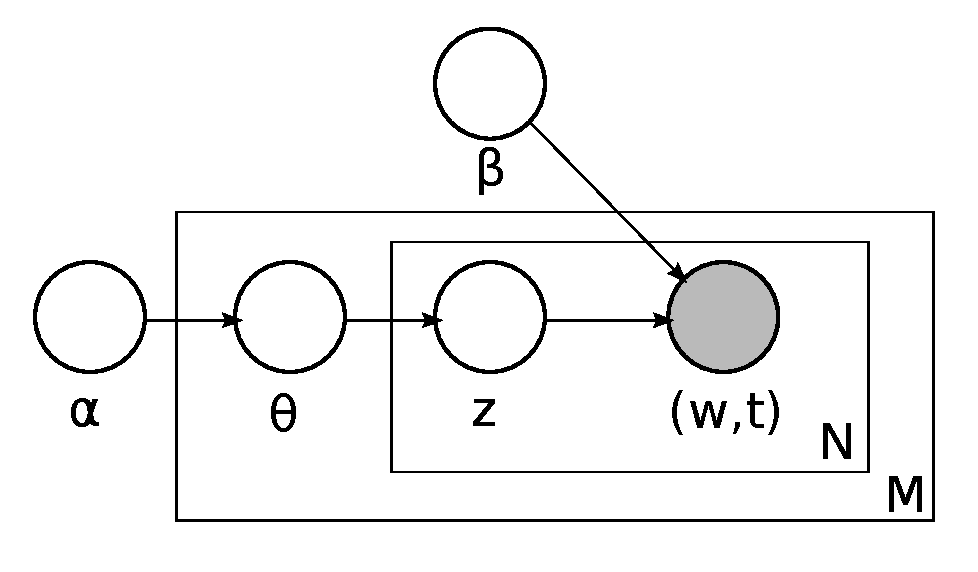
\includegraphics[width=\linewidth]{LDA.pdf}
%\caption{Latent Dirichlet allocation adapted to generate truth values.}
%\label{figure:lda}
%\end{figure}
%
%Figure \ref{figure:lda} shows how LDA can be adapted to generate truth
%values and words simultaneously. The probability of a word, truth
%value pair $(w,t)$ being generated is conditioned on the topic $z$
%generated for that word; in standard LDA only a word is generated. The
%rest of the model remains the same.
%
%If we consider words as sentences and documents as theories, then,
%this ``truth value LDA'' can be viewed as an instance of our
%Stochastic Semantics.

\section{Intermediate Models}

In this section, we show how the expressivity and complexity of
probabilistic Montague semantics can be reproduced within stochastic
semantics by increasing the number of hidden variable values $H$. This
allows us to trade expressivity for reduced complexity by varying the
size of $H$. We will show that probabilistic Montague semantics can be
expressed as a special case of stochastic semantics.

Given a probabilistic Montague semantics with parameters $\theta$, we
construct an equivalent stochastic semantics. First we define a new
set of hidden variables,
$$H' = H \times \prod_{b\in B} H_b \times \prod_{\alpha,\beta}
H_{\alpha,\beta}$$ where $H$ is the set of hidden values in the
original probabilistic Montague semantics, $\prod$ denotes the
Cartesian product and $\alpha$ and $\beta$ range over values such that
$\alpha/\beta$ is the type of a well formed expression. Each $H_b$ has
an element for each value that the denotation of the basic expression
$b$ can take,
$$H_b = \{h_{b,0}, h_{b,1},\ldots h_{b, n_{\tau_b}}\}$$
Each $H_{\alpha,\beta,i,j}$ has $n_\alpha$ elements, one for each
value that $d_{\alpha/\beta,i}(d_{\beta,j})$ can take:
$$H_{\alpha,\beta,i,j} = \{h_{\alpha,\beta,i,j,0}, h_{\alpha,\beta,i,j,1},\ldots h_{\alpha,\beta,i,j,n_{\alpha}}\}$$

We now define probability distributions $\theta'$ for stochastic
semantics to reproduce the equivalent of $\theta$ in probabilistic
Montague semantics. Here $\theta_h'$ contains most of the complexity,
and reproduces the probability distribution of probabilistic Montague
semantics, while the remainder of $\theta'$ is used to enforce the
constraint that each basic expression and denotation must take the
same value within an interpretation.
%% Each $h'\in H'$ can be written
%% $h' = (h, 

\section{Discussion}

\begin{table}
  \begin{center}
    \begin{tabular}{l|l|l}
      Text & Hypothesis & Ent.\\
      \hline
      some cats like all dogs & some animals like all dogs & Yes\\
      no animals like all dogs & no cats like all dogs & Yes\\
      some dogs like all dogs & some animals like all dogs & Yes\\
      no animals like all dogs & no dogs like all dogs & Yes\\
      some men like all dogs & some people like all dogs & Yes\\
      \hline
      no people like all dogs & no men like all dogs & Yes\\
      no men like all dogs & no people like all dogs & No\\
    \end{tabular}
    \vspace{0.2cm}
    \caption{Example Text and Hypothesis sentences, and whether
      entailment holds. Both our systems are able to learn from the
      data above the line that the determiner ``no'' reverses the
      direction of entailment.}
    \label{table:mono}
  \end{center}
\end{table}

\begin{table}
  \centering

\csvreader[tabular=l|l|l|l,
  table head=Noun & Hidden & n0 & n1\\\hline,
  head to column names]%
{lexical.csv}{}{\Noun & \Hidden & \nzero & \ntwo}

%% {}%
%% {\thecsvrow & \surname~\name & \age}%
  %% \csvautotabular{lexical.csv}
  \vspace{0.2cm}
  \caption{Learnt probabilities obtained using the
    Stochastic Semantics implementation.}
  \label{table:lexical-sato}
\end{table}

A learning system such as those we have described can be adapted to
the task of recognising textual entailment \cite{Dagan:05}. This task is
to determine whether one natural language sentence (the ``text'')
entails another (the ``hypothesis'') and thus generalizes some
important natural language problems, including question answering,
summarisation and information extraction.  For example, a pair for
which entailment holds could be translated to the following set of
theories:
\[
\{(s_T,\top),(s_H,\top)\},  \{(s_T,\bot),(s_H,\top)\},\{(s_T,\bot),(s_H,\bot)\}
\]
where $s_T$ is the sentence associated with the text and $s_H$ the
sentence associated with the hypothesis.


We verified that our two systems were able to learn some simple
logical features of natural language semantics on toy textual
entailment examples. In particular, determiners such as ``no''
reverse the direction of entailment, so that while ``some cats''
entails ``some animals'', ``no animals'' entails ``no cats'' (see Table
\ref{table:mono}). As an aside, we note that while our formalism does not employ explicit representations of lexical semantics, such representations can be recovered from the learnt models. The representation of a word is a tensor rather than a vector, because there is a distinct probability distribution over possible values for each hidden value. Table \ref{table:lexical-sato} shows the learnt values for the nouns obtained using the Stochastic Semantics implementation. 
%Allowing the distribution to vary with the hidden variable is precisely what enables learning of the behaviour of quantifiers. Without this flexibility learning would not be possible. 
If we want to compare words 
%in a manner similar to vector based
%representations of meaning, 
we can consider the matrix entries as a
flat vector and use any of the standard similarity measures (e.g. 
cosine).
%to compare word representations.


%The two models of semantics we have discussed are closely
%related.
% It is notable that Sato's framework is also based around a probability
% distribution over models. However, because of its foundation in logic
% programming, only \emph{Herbrand} models are considered.
%The semantics
%of the switches in the PRISM language means that they are assigned
%a random value on each evaluation. This is why a term may have different meanings
%within a single interpretation. In contrast, the model based on
%Montague semantics would require switches to take the same value on
%each evaluation, which is not directly supported by PRISM.

The flexibility granted by Stochastic Semantics results in the loss of certain nice properties. 
%
%For Probabilistic Montague Semantics, it is easy to verify that any given sentence must entail itself to degree 1. This is no longer guaranteed in our model of Stochastic Semantics. 
%
%Indeed 
%
A necessary consequence of incorporating stochastic ambiguity into the formalism is the failure of logical entailment.
%In standard model-theoretic semantics, it may be assumed that sentences are disambiguated before any reasoning is performed. 
If we do not disambiguate, then a sentence may not entail itself to degree 1 since it may mean different things in different contexts. We argue that it makes sense to sacrifice some properties which are expected when handling logical expressions in order to account for ambiguity as as an inherent property of language.

It is notable that the approach that accounts for ambiguity has lower
complexity.
Intuitively, this is because we
do not have to keep track of the interpretation previously assigned to
an expression: we are free to assign a new one. This also means that the expressive power of Probabilistic Montague
Semantics is greater than that of Stochastic Semantics. In the latter, the
meaning of a sentence can be viewed as simply a distribution over
hidden variables, whereas in the former, the meaning also
includes, for example, a record of all the words contained in the
sentence.
It is possible that Probabilistic Montague Semantics can be made more
computationally efficient by placing further restrictions on the
nature of distributions over models. For example, if we have no hidden
variables, then the distribution
can be described efficiently using Markov Logic Networks. Again, this
restriction comes at the expense of expressive power.

% We note too that the two models also have different computational properties.
% In particular, Stochastic Semantics allows for efficient computation with dynamic
% programming. This is possible because of the re-evaluation of switch
% values: each evaluation is independent of previous ones. In contrast,
% in Probabilistic Montague Semantics, we need to remember choices made
% previously, which means we lose the independence property in general,
% making dynamic programming much less useful. 



% \subsection{Application to Textual Entailment}

% The task of recognising textual entailment \cite{Dagan:05} is to
% determine, given two sentences $T$ (the \emph{text}) and $H$ (the
% \emph{hypothesis}), whether $T$ {\em textually entails\/} $H$. It is important to note that the notion of
% textual entailment is an informal one based on human judgments. This makes textual entailment much closer to the notion of degree of entailment available within our probabilistic approach than that of strict logical entailment.  The importance of textual entailment within natural language processing lies in its broad relevance to a range of tasks. It represents a core problem, a solution to which is required in order to develop applications in areas such as
% information retrieval, machine translation, question answering and
% summarisation.

% Previous attempts to apply logical representations of meaning to this
% task have applied {\em ad hoc\/} heuristics to handle the lack of robustness in
% standard approaches. \citet{Bos:06} used model builders to construct a
% model for $T$ and a model for $T$ and $H$ together and used the size
% of these models as an indication of the degree of entailment. The
% intuition here is that if the model for $T$ and $H$ together is larger
% than that for just $T$, then $H$ contains a lot of knowledge not in
% $T$ and there is a low degree of entailment.  This idea can be
% directly related to our approach: it amounts to assuming the existence of a probability
% distribution over models,
% with larger models less probable than smaller ones.

% Textual entailment datasets can also be used to learn the parameters
% described in the previous section. A dataset typically consists of a
% set of natural language sentence pairs, each annotated as to whether
% entailment holds or not. Suppose we are given a pair $(T,H)$ with associated meaningful expressions $s_T$ and $s_H$. In the case that entailment holds for $T$ and $H$ then the dataset will contain the following theories as observations:
% \[
% \{(s_T,\top),(s_H,\top)\}, \{(s_T,\bot),(s_H,\top)\},\{(s_T,\bot),(s_H,\bot)\}
% \]
% In the case that entailment does not hold, on the other hand, then the dataset will contain just the following as an observation:
% \[
% \{(s_T,\top),(s_H,\bot)\}
% \]

% This
% idea could be used as a supervised approach to the general task of recognising textual
% entailment.  However, we leave the evaluation of this idea to future
% work.

\section{Related Work}

%\cite{Clarke:07,Coecke:10,Garrette:11,Lewis:13}. 

\newcite{Eijck:12} presents a framework for probabilistic semantics that is motivated by the need to account for gradience effects as an intrinsic part of a model of linguistic competence. They outline a compositional semantics for a propositional language in which the probability of the truth of a sentence is defined in terms of a probability distribution over possible states of affairs (worlds). Whilst the importance of providing a computationally adequate explanation of semantic learning is emphasised, issues of the tractability of inference are not addressed. 

In a computational setting, an important objection to the appeal to possible worlds is that they are not tractably representable. \newcite{Cooper:14}  proposes a rich type system with records in which the judgment about whether a given situation is of a given type is probabilistic. Unlike worlds, situation types~\cite{Barwise:83} are not maximal consistent sets of propositions, but may be as small or as large as necessary. A schematic theory of semantic learning is outlined, based on an individual's observations of situations and their types, modelled probabilistically. This account of meaning provides the basis for a compositional semantics employing a probabilistic interpretation function. 

In contrast to \cite{Cooper:14}, the present work assumes a generative process over interpreting structures. In particular, this means that interpretation with respect to a given model is categorical, while meaning is defined in terms of the probability distribution over all models. By restricting the space of possible models we show that semantic learning is possible, where the primary data for learning are pairs of sentences and truth values (rather than probabilistic type judgments). A result of our learning is the ability to determine degrees of entailment between pairs of sentences.

The present work shares motivation with \newcite{Goodman:14}, who argue for the role of uncertainty in cognition and language understanding whilst preserving a compositional, truth conditional semantics. They show how probability may be used to formalise uncertainty and the gradience of judgements about belief and inference. The approach introduces a stochastic $\lambda$-calculus to provide compositional tools for probabilistic modelling,
but has not yet addressed the problem of learning.

Coecke et al.~\cite{Coecke:10} propose a framework based on category-theoretic
similarities between vector spaces and pregroup grammars. Their
approach is closely related to ours since it is also
founded in Montague semantics: words are treated as linear functions
between vector spaces. 
Each word is represented as an element of a
tensor product space, and a pregroup grammar is used to determine how
these are composed using the inner product. It was recently
demonstrated that this approach can be extended to allow the
simulation of predicate calculus using
tensors \cite{Grefenstette:13}.

There are two main differences between their approach and ours. First,
in the language of Montague semantics, they assume a single
model. This means that composition necessarily loses information about
the composed words, and this is evident in the use of the inner
product for composition. Sentences are all described in a space of
fixed dimensionality, no matter how long or complex they are. In our
approach, a sentence describes a probability distribution over models,
which is an infinite set, allowing for the representation of arbitrary
complexity. The second difference is that their approach is vector-based whereas
ours is probabilistic in nature. Thus their approach is more
closely related to approaches to lexical distributional semantics
which are vector based, such as latent semantic analysis
\cite{Deerwester:90} and random indexing \cite{Sahlgren:02}, whereas
ours is closer to probabilistic approaches such as latent Dirichlet
allocation \cite{Blei:03}.

\newcite{Garrette:11} describe an approach to combining logical
semantics with distributional semantics using Markov Logic Networks
\cite{Richardson:06}. Sentences are parsed into logical form using
Boxer \cite{Bos:04} and probabilistic rules are added using the
distributional model of \newcite{Erk:10}. \newcite{Lewis:13} take a standard logical approach to
semantics except that the relational constants used are derived from
distributional clustering. 
They use latent Dirichlet allocation to
describe a probability distribution over semantic categories for
nouns. These are then combined with induced relation clusters to
generate a probability distribution over logical forms for a given
sentence.

\section{Conclusion}

This paper has explored theoretical properties of models of meaning. The
reader may question the value of a paper whose contributions
are mainly theoretical in nature. Whilst we fully intend to further explore
our ideas in an experimental setting, we believe that readers
interested in probabilistic approaches to natural language semantics
will benefit from the theoretical ideas presented here. In particular:

\begin{itemize}
\item We take a standard approach to natural language semantics
  (Montague semantics) and augment it using a standard approach
  (probabilistic semantics). We are thus in an area that seems natural
  to explore.
\item We are able to demonstrate deficiencies of this approach, both
  in representational adequacy and computational complexity, that may provide
  useful guidance for others considering venturing into this
  landscape.
\item We identify an alternative area for exploration that alleviates
  the difficulties associated with the first approach.
\end{itemize}

We have shown that:

\begin{enumerate}
\item It is possible to learn probability
  distributions over models directly from data by restricting the set of models,
  whilst retaining many of the desirable properties of full Montague
  semantics.
\item The problem of computing the probability that a
  sentence is true in this framework is NP-hard.
\item Taking account of lexical ambiguity suggests a new
  approach in which pairs of sentences and truth values are generated
  randomly. The probability that a sentence is true can then be
  computed in polynomial time.
\item Both models are able to learn from a few examples
  that quantifiers such as ``no'' reverse the direction of entailment.
\end{enumerate}

%We have presented two models for probabilistic semantics for natural
%language. The first of these is a generalisation of Montague semantics
%which assumes a distribution over models. We showed how restricting
%the space of models makes it feasible to learn semantic
%representations directly from data. The second model, Stochastic Semantics, allows for the ambiguity of
%natural language expressions to be handled naturally, whilst
%sacrificing some properties of logical semantics.
%
%In the first model, the problem of computing the probability of a
%sentence is NP-hard with respect to the length of a sentence, whilst
%in the second model the computation time is linear in the sentence
%length.

% We have introduced probabilistic semantics for natural language, a
% framework for representing natural language meaning which extends
% Montague semantics by assuming a probability distribution over
% models. We have explored some properties of the framework, showing
% that it can represent fine-grained aspects of meaning, and that nice
% features of standard model-theoretic semantics, such as the simple
% representation of conjunction and disjunction are retained in our
% formalism.

% We also presented a restricted version of the semantics which makes it
% possible to learn meaning representations directly from data, and
% demonstrated that this formalism can learn the monotonicity of
% determiners from examples. We plan to apply this to practical tasks
% such as recognising textual entailment in future work.

In future work, we plan to apply our ideas to the general task of recognising textual entailment. 
This would involve learning from much larger datasets and provide a more stringent test of the practical application of the approach.
We also plan to further investigate the relationship between our models and vector space representations of meaning. This, together with a development of the theory, may lead to interesting new ways to describe probabilistic semantics that combine logical aspects of meaning with those which are better represented distributionally. 

We have so far restricted ourselves to Montague semantics, and we are
thus constrained by the well-known limitations of this formalism with
respect to expressing aspects of discourse. It would be interesting to
investigate how well our ideas could be incorporated into a formalism
such as Discourse Representation Theory.

Finally, the examples presented here deal with a very small fragment
of natural language. There are many complex natural language phenomena
that have been dealt with successfully within the framework of
Montague semantics. This suggests that it should be possible to apply
probabilistic semantics to learn about a wide range of phenomena such
as quantifier scope ambiguity, intensional contexts, time and tense
and indexicals, amongst others.

% There are a number of directions in which the work may be developed. We are currently  exploring the application of probabilistic semantics to the general task of recognising textual entailment. This would involve learning from much larger datasets and provide a more stringent test of the practical application of the approach. More work is also needed to explore the properties of the distributional representations for words that are learnt by the model. 


\bibliographystyle{fullname}
%% \bibliographystyle{acl}
\bibliography{JW2012}
\end{document}
